\documentclass{beamer}

% Opciones de lenguaje usando polyglossia (defino dos para este documento)
\usepackage{polyglossia}
\setmainlanguage{spanish}
\setotherlanguage[variant=american]{english}
\usepackage{amssymb} % Los simbolos el los conjuntos numéricos

% Poner los links en azul
\definecolor{links}{HTML}{04A3C6}
\hypersetup{colorlinks,linkcolor=,urlcolor=links}

\usepackage{graphicx} % Incluir imágenes
\usepackage{subcaption} % Poder usar subfiguras

% Tablas con estilo profesional
\usepackage{booktabs}

% Para usar varias columnas
\usepackage{multicol}

% Para poner algortmos en pseudo código
\usepackage{algpseudocode}
\usepackage{algorithm} %Ambiente flotante para los algoritmos
% \makeatletter
% \renewcommand{\ALG@beginalgorithmic}{\small}
% \makeatother


\usepackage[newfloat=true]{minted} %Para insertar código fuente en algún lenguaje de programación
% Requiere que comiples usando:
% $xelatex -shell-escape input.tex

% Configuracion del entorno minted para poner código fuente
\DeclareCaptionFormat{mitedFormat}{%
    \textbf{#1#2}#3}
\DeclareCaptionStyle{minetdStyle}{skip=0cm,width=.85\textwidth,justification=centering,
  font=footnotesize,singlelinecheck=off,format=mitedFormat,labelsep=space}
\newenvironment{mintedCode}{\captionsetup{type=listing,style=minetdStyle}}{}

\usepackage{dirtytalk} %For using qutation marks (usa comillas in spanish)

% Cambia el nombre de la etiqueta. Afecta a todos los codigos minted del codumento
\SetupFloatingEnvironment{listing}{name=Código}
% Opciones de minted para el lenguaje C++
\setminted[cpp]{frame=lines,framesep=0.25cm,baselinestretch=1,fontsize=\scriptsize,breaklines}
% Cuando lo hagas dentro de un parrafo el tamaño de fuente debe ser normal
\setmintedinline[cpp]{fontsize=auto}

\usetheme{default}

% Crear un comando con el nombre de la UNAM
\newcommand{\unam}{
  \bfseries
  \normalsize{Universidad Nacional Autónoma de México}
}

% Crear un comando para el departamento
\newcommand{\department}[1]{
    \vspace*{0.2cm}
    \bfseries
    \normalsize{#1}
}

% Crear un comando para el email
\newcommand{\email}[1]{
    \texttt{
      \href{mailto:#1}{#1}
    }
}

%Information to be included in the title page:
\title[La revolución]{Mis años en la Revolución Mexicana}
\subtitle{Una historia personal}
\author[Pancho Villa]{José Doroteo Arango Arámbula}
\institute[FES Acatlán]{
%     email for contact
    \normalsize{\email{panchovilla@unam.mx}}
    \newline
%     Department Name
%    \department{Matemáticas Aplicadas y Computación}
    \newline
%    university name
    \unam
}
\date[CONSOL 2021] % (optional)
{Congreso Nacional de Software Libre, Abril 2021}


\begin{document}

% Primer slide contiene el título
\begin{frame}{}
    \maketitle
\end{frame}

% Segundo slide el índice
\begin{frame}{Agenda}
    \begin{multicols}{2}
        \tableofcontents
    \end{multicols}
\end{frame}

\section{Antecedentes}
 \begin{frame}{¿Para que sirve?}
%     itemize
     Esta plantilla puede servir para:
     \begin{itemize}
         \item Presentar en una conferencia o evento
         \item Donde es hay varios ponentes
         \item No todo mundo te conoce.
     \end{itemize}
% 
     \vspace{0.4cm} % vertical space
%     
%     enumeration
     Para utilizar esta plantilla debes tener
     \begin{enumerate}
         \item Conocimientos mínimos de \LaTeX{}
         \item Leer el código fuente y el pdf al mismo tiempo
         \item Leer el la \href{https://github.com/nemediano/latexPlantillaUnam/blob/main/Notas/README.md}{documentación}
     \end{enumerate}
% 
     \vspace{0.2cm}
% 
%     \example{Este es un texto de ejemplo} \emph{¡Este es un texto con enfasis!}
 \end{frame}

\subsection{Formato basico} 
\begin{frame}
\frametitle{Usando columnas}
\begin{columns}
\column[t]{0.5\textwidth}
     Esta es la primer columna
     \begin{itemize}
         \item Un poco de texto
         \item Un poco mas de texto
         \item El último texto
     \end{itemize}
\column[t]{0.5\textwidth}
     Segunda columna, notese que estan alineadas hacia arriba
     \begin{enumerate}
         \item Primer punto
         \item Segundo punto
         \item Tercer punto
     \end{enumerate}
\end{columns}
\end{frame}

\begin{frame}
\frametitle{Tipos de texto}
  \begin{itemize}
    \item En negritas (bf):  \textbf{Texto de ejemplo}
    \item En italicas (it) \textit{Texto de ejemplo}
    \item En slanted (sl) \textsl{Texto de ejemplo}
    \item En tipo de letra romana (rm) \textrm{Texto de ejemplo}
    \item En tipo de fuente san serif (sf) \textsf{Texto de ejemplo}
    \item En tipo de terminal (tt) \texttt{Texto de ejemplo}
    \item En color \textcolor{orange}{Texto de ejemplo}
    \item En alerta \alert{Texto de ejemplo}
    \item En estructura \structure{Texto de ejemplo}
  \end{itemize}
\end{frame}

\subsection{Añadir elementos}
\begin{frame}
\frametitle{Una imagen desde un archivo}
\begin{figure}[htb]
  \centering
  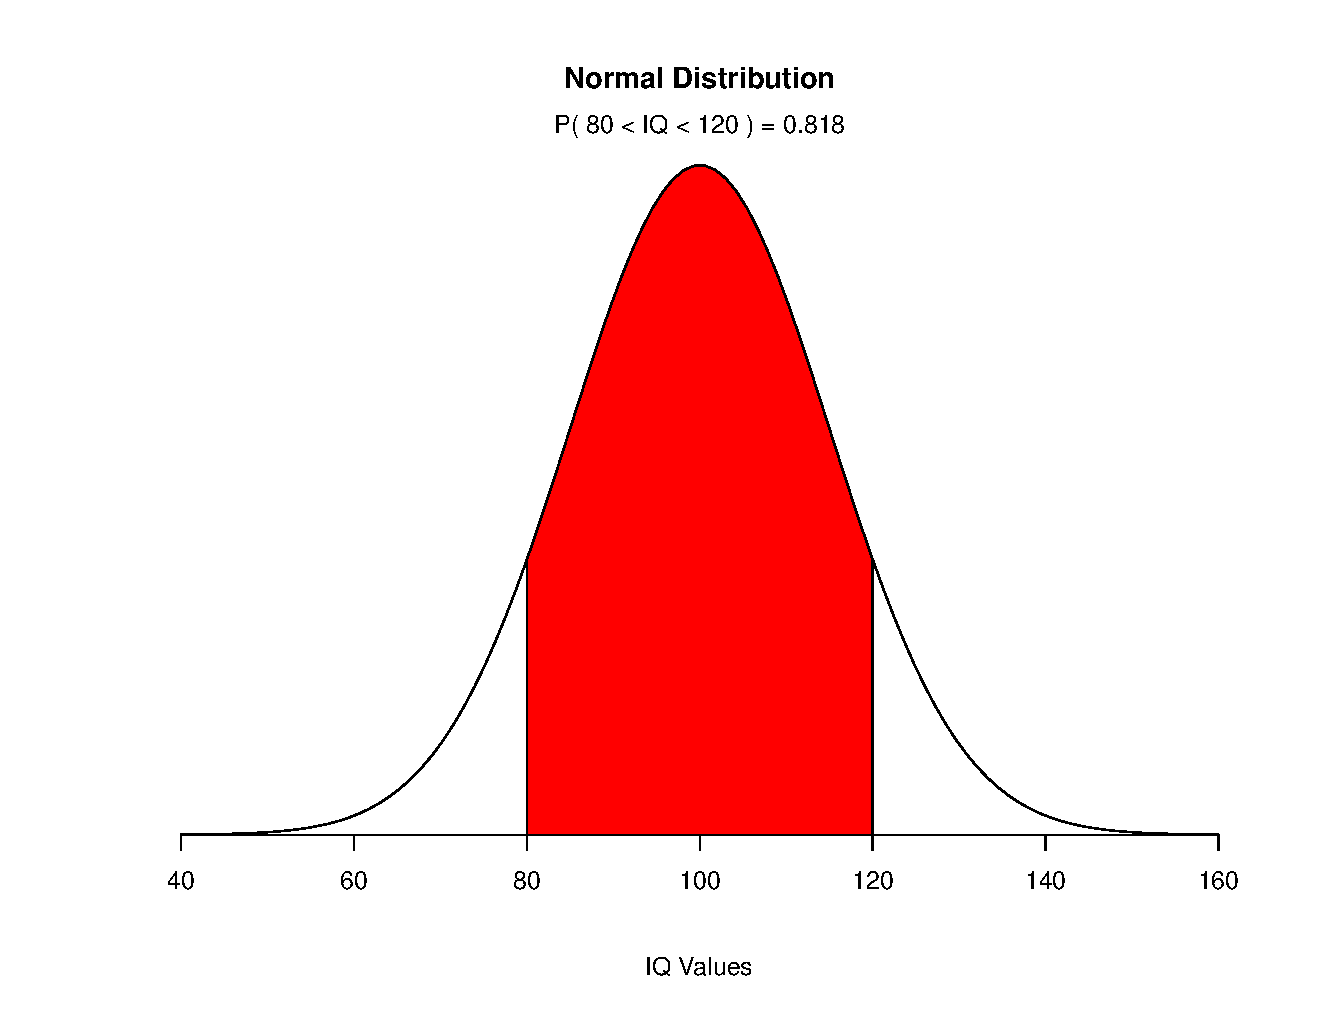
\includegraphics[width=0.70\textwidth]{img/normal}
\caption[Distribución normal]{Gráfica de una distribución normal. Fue creado usando el siguiente \href{https://www.statmethods.net/advgraphs/probability.html}{script en R}.}
\end{figure}
El caption y el resto del texto tienen la misma fuente
\end{frame}

\begin{frame}
\frametitle{Figura usando columnas}
\begin{columns}
\column[t]{0.5\textwidth}
 \begin{figure}[htb]
  \centering
  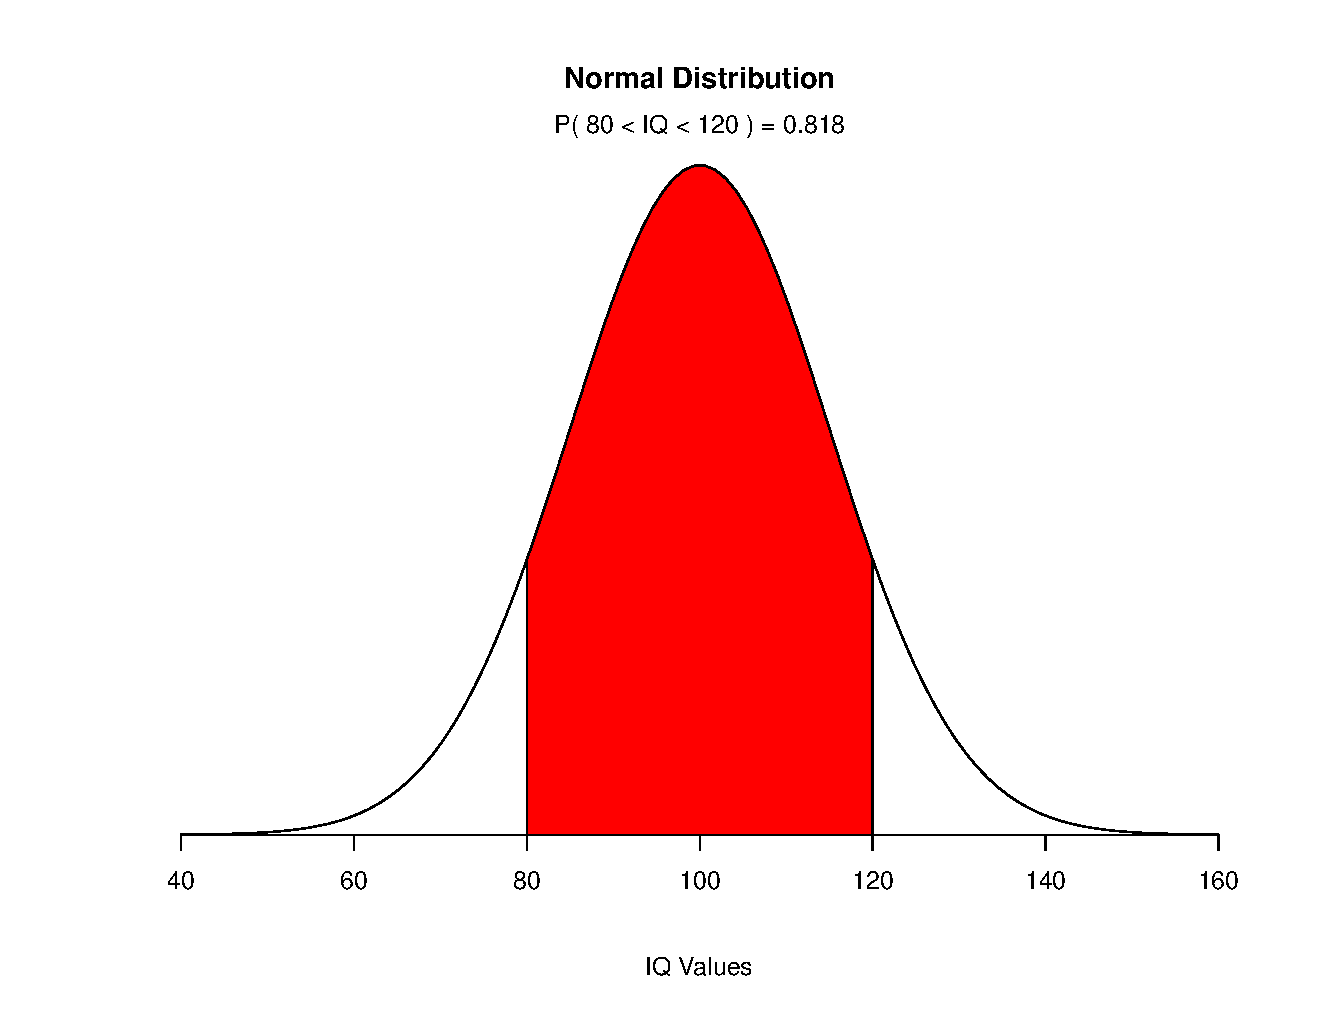
\includegraphics[width=\textwidth]{img/normal}
\caption{Gráfica de una distribución normal. Fue creado usando el siguiente \href{https://www.statmethods.net/advgraphs/probability.html}{script en R}.}
\end{figure}    
\column[t]{0.5\textwidth}
     Texto para describir la imagen
     \begin{enumerate}
         \item Se usan columnas
         \item La figura cambia de tamaño
         \item El caption puede apachurarse
     \end{enumerate}
\end{columns}
\end{frame}

\begin{frame}
\frametitle{Incluir tablas}
Este es un ejemplo de una tabla muy elegante.
Hace uso del paquete \href{https://ctan.org/pkg/booktabs}{booktabs} por que las tablas predeterminadas en \LaTeX se ven muy anticuadas.
Debes de consultar este \href{https://jdhao.github.io/2019/08/27/latex_table_with_booktabs/}{post} y leer esta \href{https://people.inf.ethz.ch/markusp/teaching/guides/guide-tables.pdf}{presentacion} si vas a usar muchas tablas.
Este ejemplo también demuestra como poner \say{comillas} en \LaTeX{}
\begin{table}[htb]
  \begin{center}
    \begin{tabular}{l | r r r r r}
      \toprule
      Source & \textbf{DF} & \textbf{SS} & \textbf{MS} & \textbf{F} & \textbf{P-value} \\
      \midrule
      \textbf{Model} & 2 & 0.00318564 & 0.00159282 & 7.72 & 0.0014 \\
      \textbf{Error} & 42 & 0.00866760 & 0.00020637 &  & \\
      \midrule
      \textbf{Total} & 44 & 0.01185324 &   &  & \\
      \bottomrule
    \end{tabular}
  \end{center}
\caption{Tabla ANOVA de un ejercicio imaginario}
\end{table}
\end{frame}

\section{Entornos de bloque}
\begin{frame}
\frametitle{Los entornos de bloque}
    % Blocks styles
    \begin{block}{Bloque generico}
        Texto dentro del bloque.
    \end{block}

    \begin{alertblock}{Bloque de Alerta}
        Texto dentro del bloque.
    \end{alertblock}

    \begin{exampleblock}{Bloque de Ejemplo}
        Texto dentro del bloque.
    \end{exampleblock}   
\end{frame}

\section{Matemáticas}
\begin{frame}
\frametitle{Incluyendo matemáticas simples}
 \begin{equation}
 \label{eq:elipse}
 \frac{x^{2}}{a^{2}} + \frac{y^{2}}{b^{2}} = 1
 \end{equation}
 
  También se pueden insertar ecuaciones dentro de un párrafo, por ejemplo: $\forall x \in \mathbb{R}$.
\end{frame}

\begin{frame}
\frametitle{Resolviendo una integral}
Un ejemplo de cómo escribir una serie de pasos matemáticos usando el entorno: \texttt{align}.
Poner $*$ dentro del entorno te permite omitir los números
\begin{align*}
P\left(X \leq 3 \right) &= \int_{0}^{3} \frac{1}{25} y \,\mathrm{d}y \\
     &= \left. \frac{1}{25} \cdot \frac{1}{2} \, y^{2} \right|_0^3 \\
     &= \frac{1}{25} \left( \frac{1}{2} \, 9 - \frac{1}{2} \, 0 \right) =
     \frac{1}{25} \cdot \frac{9}{2} = \frac{9}{50} \approx 0.18 
\end{align*}
\end{frame}

\subsection{Ciencias de la computación}
\begin{frame}
\frametitle{Incluyendo un algoritmo}
\begin{algorithm}[H]
\caption{Algoritmo de Euclides}
\label{alg:euclid}
\begin{algorithmic}[1] % El número le dice al entrono desde que numero empezar a contar. Si le pones 0 omite los números
    \Procedure{Euclid}{$a,b$} \Comment{El g.c.d. de $a$ y $b$}
    \State $r\gets a \bmod b$
    \While{$r\not=0$} \Comment{Si $r = 0$ ya tenemos la respuesta}
        \State $a \gets b$
        \State $b \gets r$
        \State $r \gets a \bmod b$
    \EndWhile\label{euclidendwhile}
    \State \textbf{return} $b$\Comment{$gcd = b$}
    \EndProcedure
\end{algorithmic}
\end{algorithm}

\end{frame}

\begin{frame}[fragile] % Usar minted requiere que uses opcion fragile
\frametitle{Incluyendo código fuente}
\begin{listing}
\begin{minted}{cpp}
int main() {
  printf("hello, world");
  return 0;
}
\end{minted}
\caption{Un programa de ejemplo en C}\label{lst:hello}
\end{listing}

Este es otro ejemplo de cómo incluir Python dentro de un párrafo: \mintinline{python}{print(x**2)}.

\end{frame}

\begin{frame}[fragile] % Usar minted requiere que uses opcion fragile
\frametitle{Incluyendo código fuente desde un archivo}
\begin{listing}
\inputminted[
  firstline=54, %If you omit this two fields, the whole file is pulled
  lastline=68
  ]{cpp}{src/GccTest.cpp}
  \caption{Una implementación defectuosa de insertion sort}\label{lst:example}
\end{listing}
\end{frame}

\end{document}
